\documentclass{beamer}
\useoutertheme{miniframes}
\useinnertheme{circles}
\definecolor{customblue}{RGB}{16,16,217}
\definecolor{redblue}{RGB}{180,16,217}
\setbeamertemplate{headline}{%
    \begin{beamercolorbox}[
        wd=\paperwidth,
        ht=3ex,dp=3ex,center
        ]{section in head/foot}

        \insertnavigation{\paperwidth}
    \end{beamercolorbox}
    \vspace{-1.2ex}%
}
\setbeamercolor{title}{fg=customblue}
\setbeamercolor{frametitle}{fg=customblue}
\setbeamertemplate{navigation symbols}{}
\setbeamertemplate{footline}{%
  \hfill%
  \usebeamerfont{footline}\usebeamercolor[fg]{footline}%
  \customblue{\insertframenumber/\inserttotalframenumber}\hspace{3mm}\vspace{3mm}
}
\setbeamercolor{itemize item}{fg=customblue}  % color for itemize
\setbeamercolor{itemize subitem}{fg=customblue}  % color for itemize
\setbeamercolor{item projected}{bg=customblue, fg=white}  % color for enumerate


\usepackage[utf8]{inputenc} % allow utf-8 input
\usepackage[T1]{fontenc}    % use 8-bit T1 fonts
\usepackage{amsmath}
\usepackage{amssymb}
\usepackage{amsthm}
\usepackage{mathtools}
\usepackage{bbm}
\usepackage[mathscr]{euscript}
\usepackage{graphicx}
\usepackage{subcaption}
\usepackage{tabularx}
\usepackage{longtable}
\usepackage{booktabs}
\usepackage{float}
\usepackage{tikz}
\usetikzlibrary{decorations.pathreplacing}
\usetikzlibrary{calc}
\usetikzlibrary{arrows.meta}
\usepackage{contour}
\usepackage[framemethod=TikZ]{mdframed}
\usepackage{xcolor}
\usepackage{caption}
\usepackage{hwemoji}
\usepackage{csquotes}
\usepackage[absolute,overlay]{textpos}
\usepackage{qrcode}
\usepackage{microtype}
\usepackage{xcolor}
\usepackage{pgfplots}
\usepackage[
    backend=biber,
    uniquename=false,
    bibencoding=utf8,
    sorting=ynt,
    doi=false,isbn=false,url=false,
    citestyle=ext-authoryear-comp,
    maxcitenames=2,
    uniquelist=false,
    maxbibnames=123,
    backref=true,
    hyperref=true
]{biblatex}
\addbibresource{references.bib}

\newcommand{\red}[1]{\textcolor{red}{#1}}
\newcommand{\blue}[1]{\textcolor{blue}{#1}}
\newcommand{\redblue}[1]{\textcolor{redblue}{#1}}
\newcommand{\customblue}[1]{\textcolor{customblue}{#1}}

% section slides
\AtBeginSection[]{
    \begin{frame}[plain,noframenumbering]
        \noindent
        \hspace*{-\dimexpr\oddsidemargin+1.1in\relax}
        \colorbox{customblue!20}{\parbox{\paperwidth}{\vspace{.2cm} \centering \usebeamerfont{caption} \LARGE \bfseries \insertsection \vspace{.2cm}}}        
    \end{frame}
}


\title{An Introduction to Tabular Foundation Models}
\author{Alexander Reisach}
\date{\today}


\begin{document}


\begin{frame}
    \titlepage
\end{frame}


\begin{frame}{Tabular foundation models}
    \begin{itemize}
        \item \textit{TabPFN} \parencite{hollmann2023tabpfn}
        \item \textit{TabICL} \parencite{qu2025tabicl}
    \end{itemize}

    \vskip1em
    \pause    
    \textbf{In-context learning setup} (tabular data $\{(X_i,Y_i)\}_{1\leq i\leq n}$)
    \begin{enumerate}
        \item \uncover<3->{split range of $Y$ into 1000 classes}
        \item \uncover<4->{pass entire dataset to a transformer}
        \item \uncover<5->{classify rows and compute avg.\ loss}
        % \item \uncover<6->{average loss across rows}
        \item \uncover<6->{perform one step of gradient descent}
    \end{enumerate}
    \vskip.5em
    \uncover<7>{Repeat for millions of (usually synthetic) datasets.}
\end{frame}


\begin{frame}{Tabular foundation models}
    \begin{minipage}{.49\linewidth}        
        Architecture (transformer-based)
        \begin{enumerate}
            \item \uncover<2->{embed each cell\\
            $(\blue{4\times 2\times d})$\\
            $(\red{3\times 1\times d})$}
            \item \uncover<3->{column-attention}
            \item \uncover<4->{add labels to features}
            \item \uncover<5->{row-attention}
            \item \uncover<6>{predict (classify) $Y$}
        \end{enumerate}
        \uncover<6>{(unlabeled cells are not attended to, and can only attend to labeled ones and themselves)}
    \end{minipage}
    \begin{minipage}{.49\linewidth}
        \begin{figure}
            \centering
            \begin{tikzpicture}
                %%%
                % \node (placeholder) at (0,-5) {$\phantom{a}$};
                % ghost copy behind the table, suggesting each cell becomes a $d$-dimensional embedding
                \node (c1a) at (1,0.5) {};
                \node (c1b) at (1,-4.2) {};
                \draw (c1a)--(c1b);
                \node (c2a) at (2,0.5) {};
                \node (c2b) at (2,-4.2) {};
                \draw (c2a)--(c2b);
                \node (r1a) at (0,-.3) {};
                \node (r1b) at (3,-.3) {};
                \draw (r1a)--(r1b);
                \node (r2a) at (0,-1.3) {};
                \node (r2b) at (3,-1.3) {};
                \draw (r2a)--(r2b);
                \node (r3a) at (0,-2.3) {};
                \node (r3b) at (3,-2.3) {};
                \draw (r3a)--(r3b);
                \node (r4a) at (0,-3.3) {};
                \node (r4b) at (3,-3.3) {};
                \draw (r4a)--(r4b);
                \node (hX1) at (.5,.2) {$X_1$};
                \node (hX2) at (1.5,.2) {$X_2$};
                \node (hY) at (2.5,.2) {$Y$};
                \only<1>{
                \node (X1R1) at (.5,-.8) {$\blue{x}_1^{(1)}$};
                \node (X2R1) at (1.5,-.8) {$\blue{x}_2^{(1)}$};
                \node (YR1) at (2.5,-.8) {$\red{y}^{(1)}$};
                \node (X1R2) at (.5,-1.8) {$\blue{x}_1^{(2)}$};
                \node (X2R2) at (1.5,-1.8) {$\blue{x}_2^{(2)}$};
                \node (YR2) at (2.5,-1.8) {$\red{y}^{(2)}$};
                \node (X1R3) at (.5,-2.8) {$\blue{x}_1^{(3)}$};
                \node (X2R3) at (1.5,-2.8) {$\blue{x}_2^{(3)}$};
                \node (YR3) at (2.5,-2.8) {$\red{y}^{(3)}$};
                \node (X1R4) at (.5,-3.8) {$\blue{x}_1^{(4)}$};
                \node (X2R4) at (1.5,-3.8) {$\blue{x}_2^{(4)}$};
                \node (YR4) at (2.5,-3.8) {};
                }
                %%%
                \only<2-3>{
                \node (X1R1) at (.5,-.8) {$\blue{\bar{x}}_1^{(1)}$};
                \node (X2R1) at (1.5,-.8) {$\blue{\bar{x}}_2^{(1)}$};
                \node (YR1) at (2.5,-.8) {$\red{\bar{y}}^{(1)}$};
                \node (X1R2) at (.5,-1.8) {$\blue{\bar{x}}_1^{(2)}$};
                \node (X2R2) at (1.5,-1.8) {$\blue{\bar{x}}_2^{(2)}$};
                \node (YR2) at (2.5,-1.8) {$\red{\bar{y}}^{(2)}$};
                \node (X1R3) at (.5,-2.8) {$\blue{\bar{x}}_1^{(3)}$};
                \node (X2R3) at (1.5,-2.8) {$\blue{\bar{x}}_2^{(3)}$};
                \node (YR3) at (2.5,-2.8) {$\red{\bar{y}}^{(3)}$};
                \node (X1R4) at (.5,-3.8) {$\blue{\bar{x}}_1^{(4)}$};
                \node (X2R4) at (1.5,-3.8) {$\blue{\bar{x}}_2^{(4)}$};
                \node (YR4) at (2.5,-3.8) {};
                }
                \only<3>{
                    % ellipsis around x_1 and x_2 to show row-attention
                    \draw[red, thick] (1,-.8) ellipse (.9 and .35);
                    \draw[red, thick] (1,-1.8) ellipse (.9 and .35);
                    \draw[red, thick] (1,-2.8) ellipse (.9 and .35);
                    \draw[red, thick] (1,-3.8) ellipse (.9 and .35);
                }
                \uncover<4->{
                    \node (X1R1) at (.5,-.8) {$\redblue{\bar{x}}_1^{(1)}$};
                    \node (X2R1) at (1.5,-.8) {$\redblue{\bar{x}}_2^{(1)}$};
                    \node (YR1) at (2.5,-.8) {$\red{\bar{y}}^{(1)}$};
                    \node (X1R2) at (.5,-1.8) {$\redblue{\bar{x}}_1^{(2)}$};
                    \node (X2R2) at (1.5,-1.8) {$\redblue{\bar{x}}_2^{(2)}$};
                    \node (YR2) at (2.5,-1.8) {$\red{\bar{y}}^{(2)}$};
                    \node (X1R3) at (.5,-2.8) {$\redblue{\bar{x}}_1^{(3)}$};
                    \node (X2R3) at (1.5,-2.8) {$\redblue{\bar{x}}_2^{(3)}$};
                    \node (YR3) at (2.5,-2.8) {$\red{\bar{y}}^{(3)}$};
                    \node (X1R4) at (.5,-3.8) {$\blue{\bar{x}}_1^{(4)}$};
                    \node (X2R4) at (1.5,-3.8) {$\blue{\bar{x}}_2^{(4)}$};
                    \node (YR4) at (2.5,-3.8) {};
                }
                \only<5>{
                    % ellipsis around each column to show column-attention
                    \draw[red, thick] (.5,-2.3) ellipse (.46 and 1.85);
                    \draw[red, thick] (1.5,-2.3) ellipse (.46 and 1.85);
                }
                \uncover<6>{
                    \node (YR4) at (2.5,-3.8) {$\hat{y}^{(4)}$};
                }
            \end{tikzpicture}
            \caption*{tabular dataset}
        \end{figure}
    \end{minipage}
\end{frame}

%%%%%%%%%%%%%%%%%%%%%%%%%%%%% Appendix %%%%%%%%%%%%%%%%%%%%%%%%%%%%%%%%%%%%%%%%%

\appendix
\newcounter{backupframenumber}
\setcounter{backupframenumber}{\value{framenumber}}

\begin{frame}[plain]
    \vskip4em
        \noindent
        \hspace*{-\dimexpr\oddsidemargin+1.1in\relax}
        \colorbox{blue!20}{\parbox{\paperwidth}{\vspace{.2cm} \centering \usebeamerfont{caption} \Huge \bfseries 
        Thank you!
        \vspace{.2cm}}}
\end{frame}

\section*{Bibliography}

\begin{frame}[allowframebreaks]{References}
    \printbibliography
\end{frame}

\setcounter{framenumber}{\value{backupframenumber}}


\end{document}